%!TEX root = practicum1.tex

\subsection{Fixed $K$}


\begin{figure}
	\centering
	\foreach \dim in {0, 1, 2}
	{ 
		\begin{subfigure}{0.3\textwidth}
			\includegraphics[width=\textwidth]{./img/assignment_a_\dim_dim.pdf}
			\caption{Buh}
			\label{fig:experiment:dimension:\dim}
		\end{subfigure}
		\begin{subfigure}{0.3\textwidth}
			\includegraphics[width=\textwidth]{./img/assignment_a_\dim_dim_progression_p.pdf}
			\caption{Progression of $p$}
			\label{fig:experiment:dimension:\dim:x}
		\end{subfigure}		
		\begin{subfigure}{0.3\textwidth}
			\includegraphics[width=\textwidth]{./img/assignment_a_\dim_dim_progression_x.pdf}
			\caption{Progression of $x$}
			\label{fig:experiment:dimension:\dim:p}
		\end{subfigure}		
	}
	\caption{}
	\label{fig:experiment:dimension}
\end{figure}


% \begin{figure}
% 	\centering
% 	\begin{subfigure}{0.9\columnwidth}
% 		\centering
% 		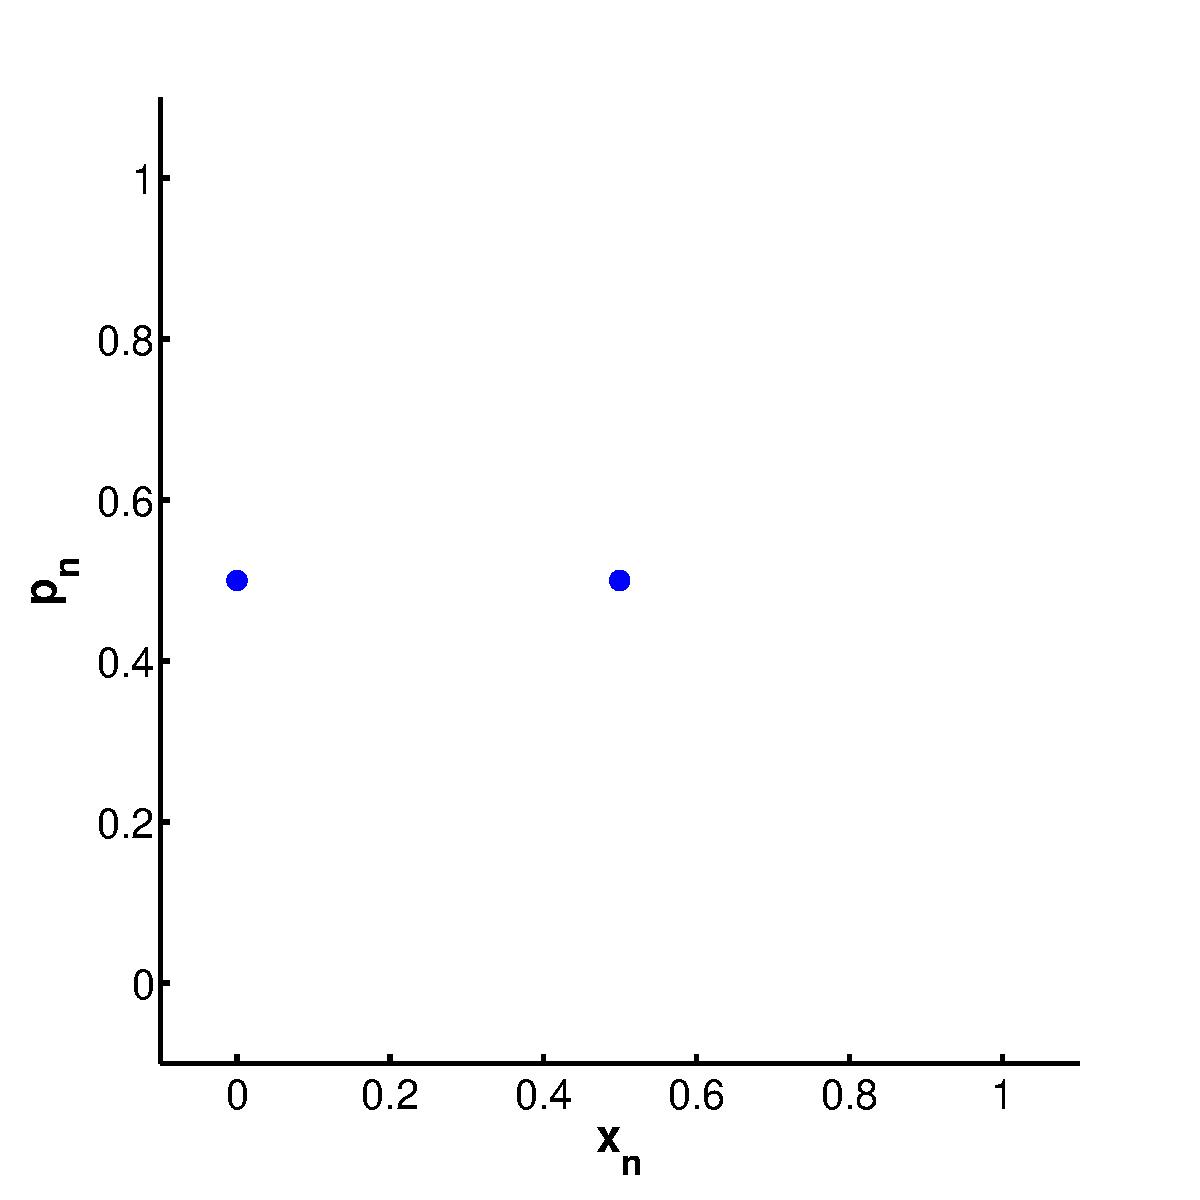
\includegraphics[width=\textwidth]{./img/assignment_a_0_dim}
% 		\caption{$x_n = 0.5, p_n = 0.5$}
% 		\label{fig:experiment:dimension:zero}
% 	\end{subfigure}

% 	\begin{subfigure}{0.9\columnwidth}
% 		\centering
% 		\includegraphics[width=\textwidth]{./img/assignment_a_1_dim}
% 		\caption{$x_n = \num{0.1576131}, p_n = \num{0.9705928}$}
% 		\label{fig:experiment:dimension:one}
% 	\end{subfigure}

% 	\begin{subfigure}{0.9\columnwidth}
% 		\centering
% 		\includegraphics[width=\textwidth]{./img/assignment_a_2_dim}
% 		\caption{$x_n = \num{0.1269868}, p_n = \num{0.9133759}$}
% 		\label{fig:experiment:dimension:two}
% 	\end{subfigure}
% 	\caption{}
% 	\label{fig:experiment:dimension}
% \end{figure}

\subsection{Variable $K$}